\documentclass{article}

\usepackage[utf8]{inputenc}
\usepackage[letterpaper, total={6in, 9in}]{geometry}
\usepackage{amsmath}
\usepackage{natbib}
\usepackage{wrapfig}
\usepackage{graphicx}
\usepackage{amssymb}
\usepackage{tikz}
\graphicspath{ {./geo3/} }

\title{Geometry 3 - Miscellaneous}
\author{TSS Math Club}
\date{Nov 2022}

\begin{document}
\large

\maketitle

\section{Pythagorean Theorem}

\begin{wrapfigure}{R}{0.4\textwidth} %this figure will be at the right
    \centering
    
    \tikzset{every picture/.style={line width=0.75pt}} %set default line width to 0.75pt        

    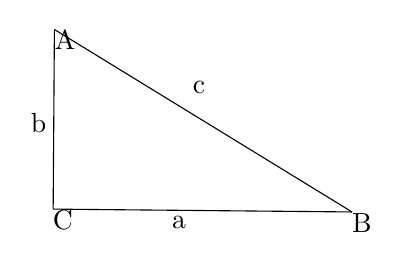
\begin{tikzpicture}[x=0.75pt,y=0.75pt,yscale=-1,xscale=1]
    %uncomment if require: \path (0,300); %set diagram left start at 0, and has height of 300

    %Straight Lines [id:da7810882093328524] 
    \draw    (99.61,122) -- (99.01,208.55) ;
    %Straight Lines [id:da0001872892319363384] 
    \draw    (99.61,122) -- (243.01,209.92) ;
    %Straight Lines [id:da14609712871080904] 
    \draw    (99.01,208.55) -- (243.01,209.92) ;

    % Text Node
    \draw (98.41,121.4) node [anchor=north west][inner sep=0.75pt]   [align=left] {A};
    % Text Node
    \draw (241.81,209.32) node [anchor=north west][inner sep=0.75pt]   [align=left] {B};
    % Text Node
    \draw (97.61,207.94) node [anchor=north west][inner sep=0.75pt]   [align=left] {C};
    % Text Node
    \draw (165,146) node [anchor=north west][inner sep=0.75pt]   [align=left] {c};
    % Text Node
    \draw (155,211) node [anchor=north west][inner sep=0.75pt]   [align=left] {a};
    % Text Node
    \draw (87,161) node [anchor=north west][inner sep=0.75pt]   [align=left] {b};


    \end{tikzpicture}

\end{wrapfigure}

In a right-triangle, 
$$a^2+b^2=c^2$$
where a and b are two sides and c is the hypotenuse.

\subsection{Proof}


\begin{minipage}{0.2\linewidth}



\tikzset{every picture/.style={line width=0.75pt}} %set default line width to 0.75pt        

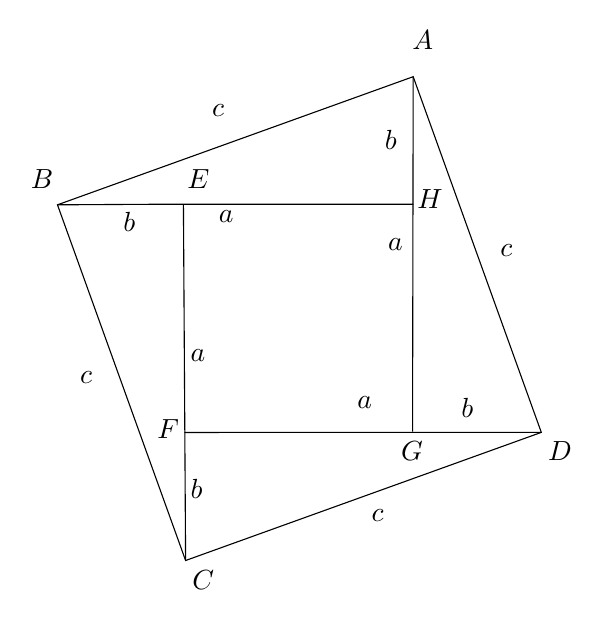
\begin{tikzpicture}[x=0.75pt,y=0.75pt,yscale=-1,xscale=1]
%uncomment if require: \path (0,300); %set diagram left start at 0, and has height of 300

%Shape: Square [id:dp7205089767241994] 
\draw   (203.92,94.48) -- (375.3,32.75) -- (437.03,204.12) -- (265.65,265.85) -- cycle ;
%Straight Lines [id:da8288112099002594] 
\draw    (203.92,94.48) -- (255.37,94.19) -- (375.4,94.2) ;
%Straight Lines [id:da929088743160273] 
\draw    (265,204.2) -- (295.4,204.11) -- (437.03,204.12) ;
%Straight Lines [id:da01808211820415795] 
\draw    (375.3,32.75) -- (375,203.8) ;
%Straight Lines [id:da6987174732927854] 
\draw    (264.6,94.2) -- (265.65,265.85) ;

% Text Node
\draw (265.2,76.2) node [anchor=north west][inner sep=0.75pt]    {$E$};
% Text Node
\draw (250.8,196.6) node [anchor=north west][inner sep=0.75pt]    {$F$};
% Text Node
\draw (373.6,9.4) node [anchor=north west][inner sep=0.75pt]    {$A$};
% Text Node
\draw (213.6,173.4) node [anchor=north west][inner sep=0.75pt]    {$c$};
% Text Node
\draw (234.4,96.6) node [anchor=north west][inner sep=0.75pt]    {$b$};
% Text Node
\draw (439.03,207.52) node [anchor=north west][inner sep=0.75pt]    {$D$};
% Text Node
\draw (376,85.8) node [anchor=north west][inner sep=0.75pt]    {$H$};
% Text Node
\draw (368.21,207.52) node [anchor=north west][inner sep=0.75pt]    {$G$};
% Text Node
\draw (267.65,269.25) node [anchor=north west][inner sep=0.75pt]    {$C$};
% Text Node
\draw (189.83,76.32) node [anchor=north west][inner sep=0.75pt]    {$B$};
% Text Node
\draw (277.2,45) node [anchor=north west][inner sep=0.75pt]    {$c$};
% Text Node
\draw (354,240.2) node [anchor=north west][inner sep=0.75pt]    {$c$};
% Text Node
\draw (416,112.6) node [anchor=north west][inner sep=0.75pt]    {$c$};
% Text Node
\draw (266.8,225.4) node [anchor=north west][inner sep=0.75pt]    {$b$};
% Text Node
\draw (397.2,186.6) node [anchor=north west][inner sep=0.75pt]    {$b$};
% Text Node
\draw (360.4,57.4) node [anchor=north west][inner sep=0.75pt]    {$b$};
% Text Node
\draw (280.4,95.8) node [anchor=north west][inner sep=0.75pt]    {$a$};
% Text Node
\draw (266.8,163) node [anchor=north west][inner sep=0.75pt]    {$a$};
% Text Node
\draw (347.2,185.4) node [anchor=north west][inner sep=0.75pt]    {$a$};
% Text Node
\draw (362,109.4) node [anchor=north west][inner sep=0.75pt]    {$a$};


\end{tikzpicture}


\end{minipage}
\hfill
\begin{minipage}{0.87\linewidth}
$[ABCD]=c^2$\\
$[ABCD]=[EFGH]+4[AEB]$\\
$[ABCD]=(a-b)^2+4\frac{ab}{2}$\\
$[ABCD]=a^2-2ab+b^2+2ab$\\
$[ABCD]=a^2+b^2$\\
Therefore, $a^2+b^2=c^2$
\end{minipage}
\pagebreak

\section{Trigonometry}

\subsection{Definitions}

Sine or $\sin(\theta)$ : A ratio between the opposite side length and the hypotenuse of a triangle.
\\ \\
Cosine or $\cos(\theta)$ : A ratio between the adjacent side length and the hypotenuse of a triangle.
\\ \\
Tangent or $\tan(\theta)$ : A ratio between the opposite side length and the adjacent side of a triangle.

\subsection{Pythagorean Theorem}
$$\sin^2 (\theta)+\cos^2 (\theta)=1$$

\subsection{Triangle Area Formula with Sine}

$$S=\frac{ab\sin C}{2}$$

\subsubsection{Proof}
Since $$\sin C=\frac{h}{b}\longrightarrow h=b\sin C$$\\
Therefore, $$S=\frac{h\times a}{2}$$
$$=\frac{\sin C\times b\times a}{2}$$
$$=\frac{ab\sin C}{2}$$
\pagebreak

\subsection{Law of Sines}

$$\frac{a}{\sin A}=\frac{b}{\sin B}=\frac{c}{\sin C}=2R=d$$

\subsubsection{Proof}
$$S=\frac{ab\sin C}{2}=\frac{bc\sin A}{2}$$
$$a\sin C=c\sin A$$
$$\frac{c}{\sin C}=\frac{a}{\sin A}$$\\

$$abc=4RS$$
$$abc=\frac{4ab\sin C}{2}R$$
$$c=2\sin CR$$
$$\frac{c}{\sin C}=2R$$
Therefore, 
$$\frac{a}{\sin A}=\frac{b}{\sin B}=\frac{c}{\sin C}=2R=d$$

\subsection{Law of Cosines}
$$c^2=a^2+b^2-2 a b \cos C $$

\subsubsection{Proof}
\begin{minipage}{0.2\linewidth}
    

\tikzset{every picture/.style={line width=0.75pt}} %set default line width to 0.75pt        

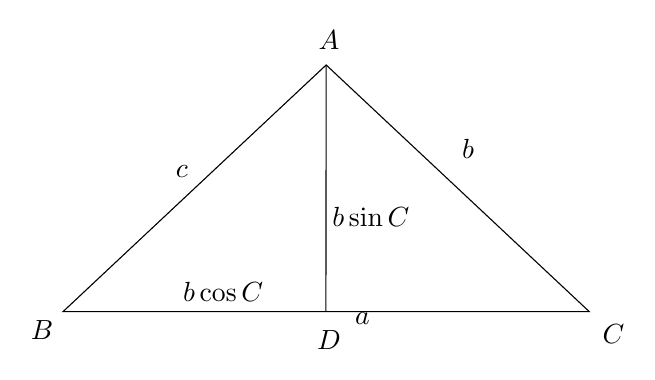
\begin{tikzpicture}[x=0.75pt,y=0.75pt,yscale=-.71,xscale=.71]
%uncomment if require: \path (0,300); %set diagram left start at 0, and has height of 300

%Shape: Triangle [id:dp2028764250879178] 
\draw   (250.17,32.33) -- (428.67,199.67) -- (71.67,199.67) -- cycle ;
%Straight Lines [id:da05842378731178721] 
\draw    (250.17,32.33) -- (250,199.33) ;

% Text Node
\draw (243.33,7.4) node [anchor=north west][inner sep=0.75pt]    {$A$};
% Text Node
\draw (48,203.73) node [anchor=north west][inner sep=0.75pt]    {$B$};
% Text Node
\draw (242.33,211.07) node [anchor=north west][inner sep=0.75pt]    {$D$};
% Text Node
\draw (436,206.4) node [anchor=north west][inner sep=0.75pt]    {$C$};
% Text Node
\draw (146.33,98.73) node [anchor=north west][inner sep=0.75pt]    {$c$};
% Text Node
\draw (268,198.4) node [anchor=north west][inner sep=0.75pt]    {$a$};
% Text Node
\draw (340.67,81.07) node [anchor=north west][inner sep=0.75pt]    {$b$};
% Text Node
\draw (151.33,178.07) node [anchor=north west][inner sep=0.75pt]    {$b\cos C$};
% Text Node
\draw (252.67,127.4) node [anchor=north west][inner sep=0.75pt]    {$b\sin C$};


\end{tikzpicture}

\end{minipage}
\hfill
\begin{minipage}{0.43\linewidth}
    $$\frac{AD}{AC}=\sin C\longrightarrow AD=b\sin C$$
    $$\frac{BC}{AC}=\cos C\longrightarrow BC=b\cos C$$
    $$DC=BC-BD=a-b\cos C$$
\end{minipage}
\begin{align*} 
c^2&=(b\sin C)^2+(a-b\cos C)^2\\
&=b^2\sin ^2C+a^2-2ab\cos C+b^2\cos ^2 C\\
&=b^2(\sin ^2 C+\cos ^2 C)+a^2-2ab\cos C\\
&=a^2+b^2-2ab\cos C
\end{align*}

\pagebreak

\subsection{Problem}
\subsubsection{Heron's Formula}
$$S= \sqrt {s (s-a) (s-b) (s-c)}, s=\frac{a+b+c}{2}$$\\
1:
\begin{align*} 
c^2&=a^2+b^2-2ab\cos C\\
\cos C&=\frac{a^2+b^2-c^2}{2ab}
\end{align*}
2: 
\begin{align*}    
\sin ^2 C+\cos ^2 C&=1\\
\sin C&=\sqrt{1-\cos ^2 C}
\end{align*}
Substitute 1 into 2: 
\begin{align*} 
\sin C&=\sqrt{1-(\frac{a^2+b^2-c^2}{2ab})^2}\\
&=\frac{\sqrt{(2ab+a^2+b^2-c^2)\times (2ab-a^2-b^2+c^2}}{2ab}\\
&=\frac{\sqrt{(a+b-c)\times (a+b+c)\times (c-a+b)\times (c+a-b)}}{2ab}
\end{align*}
Substitute into $S=\frac{ab\sin C}{2}$:
\begin{align*}
    S&=\frac{ab\sqrt{(a+b-c)\times (a+b+c)\times (c-a+b)\times (c+a-b)}}{2ab}\\
    &=\sqrt{\frac{(a+b-c)}{2}\times \frac{(a+b+c)}{2}\times \frac{(c-a+b)}{2}\times \frac{(c+a-b)}{2}}\\
    &=\sqrt{\frac{(a+b+c-2c)}{2}\times \frac{(a+b+c)}{2}\times \frac{(c+a+b-2a)}{2}\times \frac{(c+a+b-2b)}{2}}\\
    &=\sqrt{(\frac{a+b+c}{2}-c)\times (\frac{a+b+c}{2})\times (\frac{a+b+c}{2}-a)\times (\frac{a+b+c}{2}-b)}\\
    &=\sqrt{s\times (s-a)\times(s-b)\times(s-c)}
\end{align*}
\pagebreak


\subsubsection{Problem}
Given AB=3,BD=1,DC=3,AC=2. Find AD.




\tikzset{every picture/.style={line width=0.75pt}} %set default line width to 0.75pt        
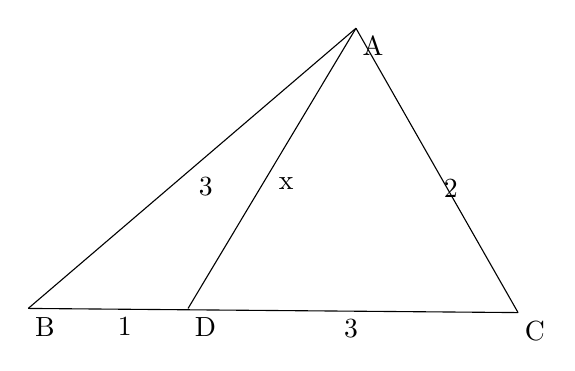
\begin{tikzpicture}[x=0.75pt,y=0.75pt,yscale=-1,xscale=1]
%uncomment if require: \path (0,389); %set diagram left start at 0, and has height of 389

%Straight Lines [id:da28332928208796315] 
\draw    (128.06,259.03) -- (364.06,261.03) ;
%Straight Lines [id:da647118791580753] 
\draw    (285.96,124.03) -- (128.06,259.03) ;
%Straight Lines [id:da4424909815278173] 
\draw    (285.96,124.03) -- (364.06,261.03) ;
%Straight Lines [id:da11044244004039627] 
\draw    (285.96,124.03) -- (205.06,259.03) ;

% Text Node
\draw (287.96,127.03) node [anchor=north west][inner sep=0.75pt]   [align=left] {A};
% Text Node
\draw (130.06,262.03) node [anchor=north west][inner sep=0.75pt]   [align=left] {B};
% Text Node
\draw (366.06,264.03) node [anchor=north west][inner sep=0.75pt]   [align=left] {C};
% Text Node
\draw (207.06,262.03) node [anchor=north west][inner sep=0.75pt]   [align=left] {D};
% Text Node
\draw (209.01,194.53) node [anchor=north west][inner sep=0.75pt]   [align=left] {3};
% Text Node
\draw (170,262) node [anchor=north west][inner sep=0.75pt]   [align=left] {1};
% Text Node
\draw (279,263) node [anchor=north west][inner sep=0.75pt]   [align=left] {3};
% Text Node
\draw (327.01,195.53) node [anchor=north west][inner sep=0.75pt]   [align=left] {2};
% Text Node
\draw (247.51,194.53) node [anchor=north west][inner sep=0.75pt]   [align=left] {x};


\end{tikzpicture}
\\\\\\
First, use cosine law to find $\angle ACD$ and $\angle ADB$:
\begin{align}
    2^2&=x^2+3^2-2(x)(3)\cos \theta\\
    4&=x^2+9-6x\cos \theta
\end{align} 
\begin{align}
    3^2&=x^2+1^2-2(x)(1)\cos 180^\circ -\theta \\
    9&=x^2+1+2x\cos \theta\\
    27&=3x^2+3+6x\cos \theta
\end{align}
Combine / add (2) and (5) together, therefore cancelling out the $6x\cos \theta$:
\begin{align*}
    4+27&=x^2+9-6x\cos \theta + 3x^2+3+6x\cos \theta\\
    31&=4x^2+12\\
    4x^2&=19\\
    x^2&=\frac{19}{4}\\
    x&=\frac{\sqrt{19}}{2}
\end{align*}
\pagebreak

\subsubsection{Problem, Euclid 2022 Q8 b)}
Consider the following statement:
\begin{quote}
There is a triangle that is not equilateral whose side lengths form
a geometric sequence, and the measures of whose angles form an
arithmetic sequence.
\end{quote}
Show that this statement is true by finding such a triangle or prove that it is false
by demonstrating that there cannot be such a triangle.\\


\tikzset{every picture/.style={line width=0.75pt}} %set default line width to 0.75pt        

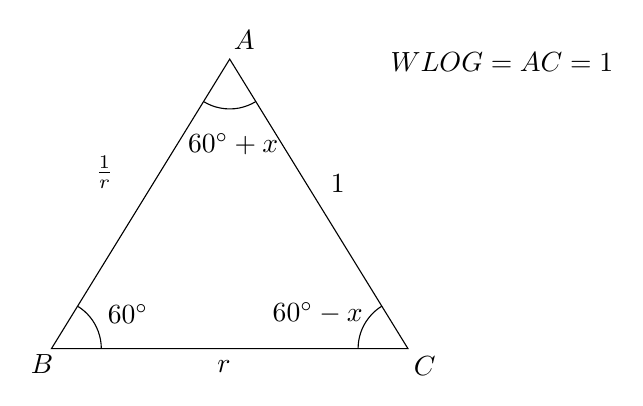
\begin{tikzpicture}[x=0.75pt,y=0.75pt,yscale=-0.8,xscale=0.8]
%uncomment if require: \path (0,300); %set diagram left start at 0, and has height of 300

%Shape: Triangle [id:dp8389982585740936] 
\draw   (362.33,51.33) -- (469.67,225.67) -- (255,225.67) -- cycle ;
%Shape: Arc [id:dp8881312346304651] 
\draw  [draw opacity=0] (271.05,200.32) .. controls (276.47,203.75) and (280.83,208.92) .. (283.19,215.41) .. controls (284.42,218.79) and (285.01,222.26) .. (285.01,225.67) -- (255,225.67) -- cycle ; \draw   (271.05,200.32) .. controls (276.47,203.75) and (280.83,208.92) .. (283.19,215.41) .. controls (284.42,218.79) and (285.01,222.26) .. (285.01,225.67) ;  
%Shape: Arc [id:dp6708474487566618] 
\draw  [draw opacity=0] (439.67,225.33) .. controls (439.73,218.93) and (441.84,212.49) .. (446.12,207.08) .. controls (448.35,204.25) and (450.99,201.93) .. (453.89,200.14) -- (469.67,225.67) -- cycle ; \draw   (439.67,225.33) .. controls (439.73,218.93) and (441.84,212.49) .. (446.12,207.08) .. controls (448.35,204.25) and (450.99,201.93) .. (453.89,200.14) ;  
%Shape: Arc [id:dp6286388230575226] 
\draw  [draw opacity=0] (378.1,76.86) .. controls (371.93,80.67) and (364.36,82.27) .. (356.67,80.79) .. controls (353.13,80.11) and (349.85,78.83) .. (346.93,77.08) -- (362.33,51.33) -- cycle ; \draw   (378.1,76.86) .. controls (371.93,80.67) and (364.36,82.27) .. (356.67,80.79) .. controls (353.13,80.11) and (349.85,78.83) .. (346.93,77.08) ;  

% Text Node
\draw (287.33,197.4) node [anchor=north west][inner sep=0.75pt]    {$60^{\circ }$};
% Text Node
\draw (386.67,196.07) node [anchor=north west][inner sep=0.75pt]    {$60^{\circ } -x$};
% Text Node
\draw (335.67,94.4) node [anchor=north west][inner sep=0.75pt]    {$60^{\circ } +x$};
% Text Node
\draw (363.33,32.73) node [anchor=north west][inner sep=0.75pt]    {$A$};
% Text Node
\draw (241,227.73) node [anchor=north west][inner sep=0.75pt]    {$B$};
% Text Node
\draw (471.67,229.07) node [anchor=north west][inner sep=0.75pt]    {$C$};
% Text Node
\draw (457.67,45.73) node [anchor=north west][inner sep=0.75pt]    {$WLOG=AC=1$};
% Text Node
\draw (421.67,119.07) node [anchor=north west][inner sep=0.75pt]    {$1$};
% Text Node
\draw (353.33,231.4) node [anchor=north west][inner sep=0.75pt]    {$r$};
% Text Node
\draw (280,108.07) node [anchor=north west][inner sep=0.75pt]    {$\frac{1}{r}$};


\end{tikzpicture}
\\\\
First, we are able to assume "Without Loss of Generality" (WLOG) since we know that changing the side lengths by a certain factor wont change its angle. Thus, we can have $AC$ as 1.\\
\begin{align*}
    \frac{\sin (60^\circ)}{1}=\frac{\sin (60^\circ+x)}{r}&=\frac{\sin (60^\circ-x)}{\frac{1}{r}}=\frac{\sqrt{3}}{2}\\
    \frac{\sin (60^\circ-x)}{\frac{1}{r}}&=\sin (60^\circ-x)\times r\\
    (\sin (60^\circ-x)\times r)\times \frac{\sin (60^\circ+x)}{r}&=( \frac{\sqrt{3}}{2})^2\\
    \sin (60^\circ-x)\times \sin (60^\circ+x)&=\frac{3}{4}
\end{align*}
Trig identities: $\sin a+b=\sin a\cos b+\cos a\sin b$ and $\sin a-b=\sin a\cos b-\cos a\sin b$ 
\begin{align*}
    (\sin 60^\circ\cos x+\cos 60^\circ\sin x)\times (\sin 60^\circ\cos x-\cos 60^\circ\sin x)&=\frac{3}{4}\\
    \frac{\sqrt{3}}{2}\cos^2 x-\frac{1}{2}\sin^2 x&=\frac{3}{4}\\
    \frac{3}{4}\cos^2 x+\frac{3}{4}\sin^2 x-\sin^2 x&=\frac{3}{4}\\
    \frac{3}{4}(\cos^2 x+\sin^2 x)-\sin^2 x&=\frac{3}{4}\\
    \frac{3}{4}-\sin^2 x&=\frac{3}{4}\\
    \sin^2 x&=0
\end{align*}
Therefore, $x=0$, and thus all three angles in the triangle are $60^\circ$, proving that no triangle exists that fit the statement provided.
\pagebreak

\section{Transversals}

\subsection{Directed Segments}
Definition: Lines with a direction.\\


\tikzset{every picture/.style={line width=0.75pt}} %set default line width to 0.75pt        

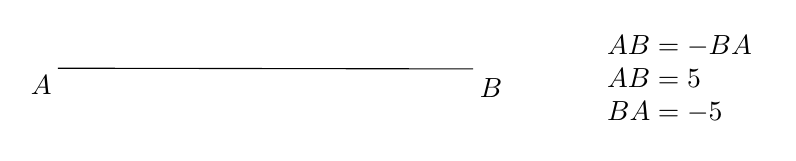
\begin{tikzpicture}[x=0.75pt,y=0.75pt,yscale=-1,xscale=1]
%uncomment if require: \path (0,300); %set diagram left start at 0, and has height of 300

%Straight Lines [id:da2454900674821967] 
\draw    (226.33,96.33) -- (426.33,96.67) ;

% Text Node
\draw (212,98.4) node [anchor=north west][inner sep=0.75pt]    {$A$};
% Text Node
\draw (428.33,100.07) node [anchor=north west][inner sep=0.75pt]    {$B$};
% Text Node
\draw (483,77.07) node [anchor=north west][inner sep=0.75pt]    {$ \begin{array}{l}
AB=-BA\\
AB=5\\
BA=-5
\end{array}$};


\end{tikzpicture}

\vspace{30px}

\subsection{Stewart's Theorem}
If A,B,C collinear and P is any other point, then
$$PA^2\cdot BC+PB^2\cdot CA+PC^2\cdot AB+BC \cdot CA \cdot AB =0$$ 



\tikzset{every picture/.style={line width=0.75pt}} %set default line width to 0.75pt        

\begin{tikzpicture}[x=0.75pt,y=0.75pt,yscale=-1,xscale=1]
%uncomment if require: \path (0,300); %set diagram left start at 0, and has height of 300

%Straight Lines [id:da5905118684092199] 
\draw    (52.91,172.03) -- (504.91,177.03) ;
%Straight Lines [id:da9618382085114188] 
\draw    (124,172) -- (233.91,52.03) ;
%Straight Lines [id:da976888364842182] 
\draw    (233.91,52.03) -- (205.91,174.03) ;
%Straight Lines [id:da13878852480396842] 
\draw    (233.91,52.03) -- (442.91,176.03) ;

% Text Node
\draw (126,175) node [anchor=north west][inner sep=0.75pt]   [align=left] {A};
% Text Node
\draw (207.91,177.03) node [anchor=north west][inner sep=0.75pt]   [align=left] {B};
% Text Node
\draw (444.91,179.03) node [anchor=north west][inner sep=0.75pt]   [align=left] {C};
% Text Node
\draw (235.91,55.03) node [anchor=north west][inner sep=0.75pt]   [align=left] {P};


\end{tikzpicture}\\
Apply cosine law in triangle $\triangle ABP$ and $\triangle CBP$ \\
\begin{equation}
\label{cos1}
AP^2 = BP^2+AB^2-2\cdot AB \cdot BP \cdot \cos(\angle ABP)
\end{equation}
\begin{equation}
\label{cos2}
CP^2 = BP^2+CB^2-2\cdot CB \cdot BP \cdot \cos(\angle CBP)
\end{equation}
(\ref{cos1}) and (\ref{cos2}) $\implies$ \\
\begin{equation}
\label{cos3}
AP^2\cdot CB = BP^2 \cdot CB +AB^2 \cdot CB -2\cdot AB \cdot BP \cdot CB \cdot \cos(\angle ABP)
\end{equation}
\begin{equation}
\label{cos4}
CP^2 \cdot AB = BP^2 \cdot AB +CB^2 \cdot AB -2\cdot CB \cdot BP \cdot  AB \cdot \cos(\angle CBP)
\end{equation}
Since $\angle ABP + \angle PBC = \pi$, (\ref{cos3}) + (\ref{cos4}) $\implies$
\begin{equation}
AP^2\cdot CB + CP^2 \cdot AB = BP^2 \cdot CB +AB^2 \cdot CB + BP^2 \cdot AB +CB^2 \cdot AB
\end{equation}
\begin{equation}
AP^2\cdot CB + CP^2 \cdot AB = BP^2 \cdot (CB+AB) +AB \cdot CB \cdot (AB+BC)
\end{equation}
\begin{equation}
\label{StewartUnsimplified}
AP^2\cdot CB + CP^2 \cdot AB = BP^2 \cdot AC +AB \cdot CB \cdot AC
\end{equation}
Checking the direction for these directed segments, (\ref{StewartUnsimplified}) implies Stewart’s Theorem.
\pagebreak

\subsection{Menelaus' Theorem}

Suppose we have a triangle ABC, and a transversal line that crosses BC, AC, and AB at points D, E, and F respectively, with D, E, and F distinct from A, B, and C, then

$$\frac{AF}{FB}\cdot \frac{BD}{DC} \cdot \frac{CE}{EA}=-1$$





\tikzset{every picture/.style={line width=0.75pt}} %set default line width to 0.75pt        

\begin{tikzpicture}[x=0.75pt,y=0.75pt,yscale=-1,xscale=1]
%uncomment if require: \path (0,300); %set diagram left start at 0, and has height of 300

%Straight Lines [id:da6022439883372588] 
\draw    (79,140.5) -- (370,141) ;
%Shape: Triangle [id:dp3107100836360235] 
\draw   (107,39) -- (209.5,140.5) -- (79,140.5) -- cycle ;
%Straight Lines [id:da16837717229751448] 
\draw    (49,49.5) -- (360,181) ;
%Straight Lines [id:da48224126119218624] 
\draw    (186,226.5) -- (214,125) ;
%Straight Lines [id:da49725778940543064] 
\draw    (214,125) -- (242,23.5) ;
%Shape: Right Angle [id:dp31614681371123354] 
\draw   (192.01,177.99) -- (200.98,173.21) -- (205.42,181.53) ;
%Shape: Right Angle [id:dp10639599189965154] 
\draw   (79.01,113.99) -- (87.98,109.21) -- (92.42,117.53) ;

% Text Node
\draw (92,21.9) node [anchor=north west][inner sep=0.75pt]    {$A$};
% Text Node
\draw (63.5,142.9) node [anchor=north west][inner sep=0.75pt]    {$B$};
% Text Node
\draw (211.5,143.9) node [anchor=north west][inner sep=0.75pt]    {$C$};
% Text Node
\draw (252,144.9) node [anchor=north west][inner sep=0.75pt]    {$D$};
% Text Node
\draw (169,79.9) node [anchor=north west][inner sep=0.75pt]    {$E$};
% Text Node
\draw (78.5,70.4) node [anchor=north west][inner sep=0.75pt]    {$F$};


\end{tikzpicture}
\\\\
Since $CG$ is parallel to $BA$, $\triangle AFE$ is similar to $\triangle CGE$, and therefore:
$$\frac{AF}{CG}=\frac{EA}{CE}=\frac{EF}{EG}$$
Since $\triangle FBD$ is similar to $\triangle GCD$, therefore:
$$\frac{GC}{FB}=\frac{DC}{BD}=\frac{DG}{DF}$$\\
We are able to multiply together certain parts of the relation listed above to get:
\begin{align*}
    \frac{AF}{CG}\times\frac{GC}{FB}&=\frac{EA}{CE}\times\frac{DC}{BD}\\
    -\frac{AF}{FB}\times(-\frac{CE}{EA}\times\frac{BD}{DC})&=(\frac{EA}{CE}\times\frac{DC}{BD})\times(-\frac{CE}{EA}\times\frac{BD}{DC})\\
    \frac{AF}{FB}\cdot \frac{BD}{DC} \cdot \frac{CE}{EA}&=-1    
\end{align*}

\subsection{Menelaus' Inverse Theorem}

Suppose we have a triangle ABC with D on BC, E on AC, F on AB, such that,
$$\frac{AF}{FB}\cdot \frac{BD}{DC} \cdot \frac{CE}{EA}=-1$$
then D,E, F collinear.\\\\


\pagebreak

\subsection{Ceva's Theorem}
Given a triangle ABC, let the lines AO, BO and CO be drawn from the vertices to a common point O (not on one of the sides of ABC), to meet opposite sides at D, E and F respectively, then

$$\frac{AF}{FB}\cdot \frac{BD}{DC} \cdot \frac{CE}{EA}=1$$



\tikzset{every picture/.style={line width=0.75pt}} %set default line width to 0.75pt        


Note:\\

\begin{minipage}{0.3\linewidth}

\tikzset{every picture/.style={line width=0.75pt}} %set default line width to 0.75pt        

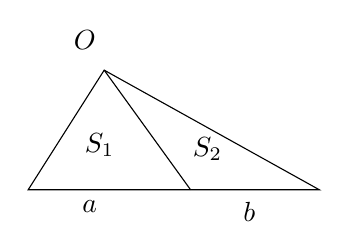
\begin{tikzpicture}[x=0.75pt,y=0.75pt,yscale=-1,xscale=1]
%uncomment if require: \path (0,300); %set diagram left start at 0, and has height of 300

%Shape: Triangle [id:dp2868878057078903] 
\draw   (76.6,45.4) -- (180.2,103) -- (40,103) -- cycle ;
%Straight Lines [id:da18136882666626764] 
\draw    (76.6,45.4) -- (118.2,103) ;

% Text Node
\draw (60.7,25.2) node [anchor=north west][inner sep=0.75pt]    {$O$};
% Text Node
\draw (64.8,107) node [anchor=north west][inner sep=0.75pt]    {$a$};
% Text Node
\draw (142.4,107.8) node [anchor=north west][inner sep=0.75pt]    {$b$};
% Text Node
\draw (66,74.8) node [anchor=north west][inner sep=0.75pt]    {$S_{1}$};
% Text Node
\draw (118,76.4) node [anchor=north west][inner sep=0.75pt]    {$S_{2}$};

\end{tikzpicture}
    
\end{minipage}
\begin{minipage}{0.8\linewidth}
    If $S_1=\frac{ah}{2}$ and $S_2=\frac{bh}{2}$, therefore $\frac{S_1}{S_2}=\frac{\frac{ah}{2}}{\frac{bh}{2}}=\frac{a}{b}$.\\
\end{minipage}
\\\\
\begin{minipage}{0.4\linewidth}

\tikzset{every picture/.style={line width=0.75pt}} %set default line width to 0.75pt        

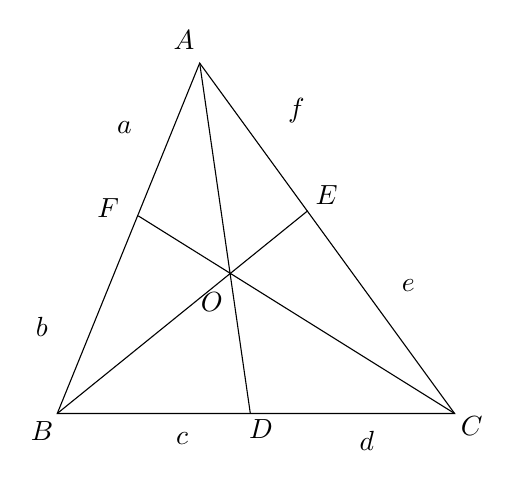
\begin{tikzpicture}[x=0.75pt,y=0.75pt,yscale=-1,xscale=1]
%uncomment if require: \path (0,300); %set diagram left start at 0, and has height of 300

%Shape: Triangle [id:dp7900101777669155] 
\draw   (280.2,54.6) -- (403,223.4) -- (211.6,223.4) -- cycle ;
%Straight Lines [id:da2657456500431752] 
\draw    (332.2,125.8) -- (211.6,223.4) ;
%Straight Lines [id:da8688743189791881] 
\draw    (280.2,54.6) -- (304.6,223.4) ;
%Straight Lines [id:da32512355801970805] 
\draw    (250.6,128.2) -- (403,223.4) ;

% Text Node
\draw (279.5,164) node [anchor=north west][inner sep=0.75pt]    {$O$};
% Text Node
\draw (229.6,118.6) node [anchor=north west][inner sep=0.75pt]    {$F$};
% Text Node
\draw (334.8,112.2) node [anchor=north west][inner sep=0.75pt]    {$E$};
% Text Node
\draw (302.8,225) node [anchor=north west][inner sep=0.75pt]    {$D$};
% Text Node
\draw (404.8,223.8) node [anchor=north west][inner sep=0.75pt]    {$C$};
% Text Node
\draw (197.6,226.2) node [anchor=north west][inner sep=0.75pt]    {$B$};
% Text Node
\draw (266.4,37.8) node [anchor=north west][inner sep=0.75pt]    {$A$};
% Text Node
\draw (239.2,81.4) node [anchor=north west][inner sep=0.75pt]    {$a$};
% Text Node
\draw (321.6,70.2) node [anchor=north west][inner sep=0.75pt]    {$f$};
% Text Node
\draw (376.4,157.4) node [anchor=north west][inner sep=0.75pt]    {$e$};
% Text Node
\draw (356,230.6) node [anchor=north west][inner sep=0.75pt]    {$d$};
% Text Node
\draw (267.6,231.4) node [anchor=north west][inner sep=0.75pt]    {$c$};
% Text Node
\draw (200,175.8) node [anchor=north west][inner sep=0.75pt]    {$b$};


\end{tikzpicture}
    
\end{minipage}
\begin{minipage}{0.5\linewidth}
    $$[BOC]=(c+d)(h/2)$$
    \begin{align}
        \frac{[BOC]}{[BOA]}&=\frac{e}{f}\\
        [BOA]&=\frac{f(c+d)(h/2)}{e}
    \end{align}
    \begin{align}
        \frac{[AOC]}{[BOC]}&=\frac{a}{b}\\
        [AOC]&=\frac{a(c+d)(h/2)}{b}
    \end{align}
    \hfill
\end{minipage}
\\
Combine (7) and (9):\\
\begin{align*}
    \frac{[AOC]}{[AOB]}&=\frac{d}{c}\\
    &=\frac{\frac{a(c+d)(h/2)}{b}}{\frac{f(c+d)(h/2)}{e}}\\
    &=\frac{a}{b}\times\frac{e}{f}
\end{align*}
Therefore,
$$\frac{d}{c}=\frac{a}{b}\times\frac{e}{f}\longrightarrow\frac{a}{b}\times\frac{c}{d}\times\frac{e}{f}=1$$
or,
$$\frac{AF}{FB}\times \frac{BD}{DC} \times \frac{CE}{EA}=1$$
\vspace{200px}

\subsection{Ceva's Inverse Theorem}

Suppose we have a triangle ABC with D on BC, E on AC, F on AB, such that,
$$\frac{AF}{FB}\cdot \frac{BD}{DC} \cdot \frac{CE}{EA}=1$$
then AD,BE,CF concurrent.

\section{Barycentric Coordinate}
\subsection{Definition}
The barycentric coordinates of a point can be interpreted as masses placed at the vertices of the simplex, such that the point is the center of mass (or barycenter) of these masses.



\tikzset{every picture/.style={line width=0.75pt}} %set default line width to 0.75pt        

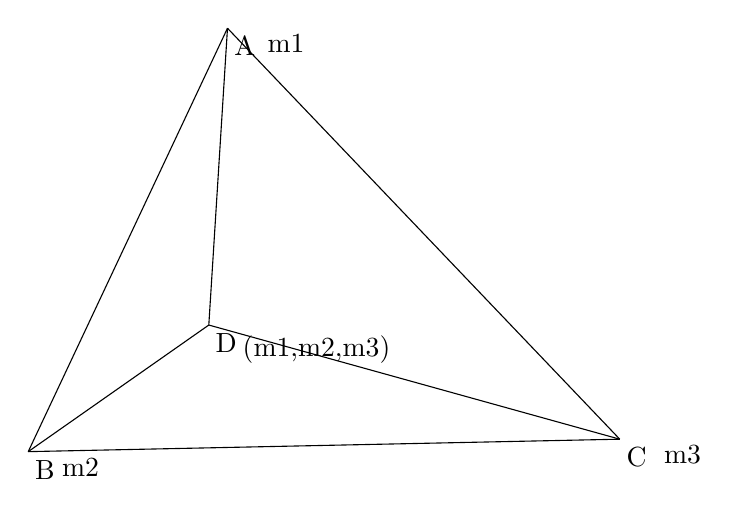
\begin{tikzpicture}[x=0.75pt,y=0.75pt,yscale=-1,xscale=1]
%uncomment if require: \path (0,300); %set diagram left start at 0, and has height of 300

%Straight Lines [id:da9034961562868877] 
\draw    (262.91,41.03) -- (166.91,245.03) ;
%Straight Lines [id:da38322702999878766] 
\draw    (451.91,239.03) -- (166.91,245.03) ;
%Straight Lines [id:da8608907326548492] 
\draw    (262.91,41.03) -- (451.91,239.03) ;
%Straight Lines [id:da9987380023335841] 
\draw    (262.91,41.03) -- (253.91,184.03) ;
%Straight Lines [id:da3386128853211863] 
\draw    (253.91,184.03) -- (166.91,245.03) ;
%Straight Lines [id:da20853567056026168] 
\draw    (253.91,184.03) -- (451.91,239.03) ;

% Text Node
\draw (264.91,44.03) node [anchor=north west][inner sep=0.75pt]   [align=left] {A};
% Text Node
\draw (168.91,248.03) node [anchor=north west][inner sep=0.75pt]   [align=left] {B};
% Text Node
\draw (453.91,242.03) node [anchor=north west][inner sep=0.75pt]   [align=left] {C};
% Text Node
\draw (255.91,187.03) node [anchor=north west][inner sep=0.75pt]   [align=left] {D};
% Text Node
\draw (281,43) node [anchor=north west][inner sep=0.75pt]   [align=left] {m1};
% Text Node
\draw (182,247) node [anchor=north west][inner sep=0.75pt]   [align=left] {m2};
% Text Node
\draw (472,241) node [anchor=north west][inner sep=0.75pt]   [align=left] {m3};
% Text Node
\draw (269,188) node [anchor=north west][inner sep=0.75pt]   [align=left] {(m1,m2,m3)};


\end{tikzpicture}


\subsection{Example}

Given BD:DC=1:2, AE:EC=1:1. Find AF:FD.\\
\begin{minipage}{0.5\linewidth}

\tikzset{every picture/.style={line width=0.75pt}} %set default line width to 0.75pt        

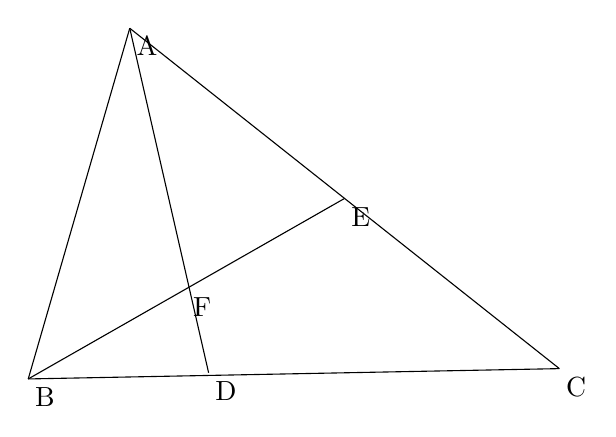
\begin{tikzpicture}[x=0.75pt,y=0.75pt,yscale=-1,xscale=1]
%uncomment if require: \path (0,300); %set diagram left start at 0, and has height of 300

%Straight Lines [id:da7675617641029677] 
\draw    (248.91,41.03) -- (200,210) ;
%Straight Lines [id:da08477900268519623] 
\draw    (248.91,41.03) -- (455.91,205.03) ;
%Straight Lines [id:da9475888247486965] 
\draw    (455.91,205.03) -- (200,210) ;
%Straight Lines [id:da019733232113179566] 
\draw    (248.91,41.03) -- (286.91,207.03) ;
%Straight Lines [id:da6042356170051348] 
\draw    (200,210) -- (352.41,123.03) ;

% Text Node
\draw (250.91,44.03) node [anchor=north west][inner sep=0.75pt]   [align=left] {A};
% Text Node
\draw (202,213) node [anchor=north west][inner sep=0.75pt]   [align=left] {B};
% Text Node
\draw (457.91,208.03) node [anchor=north west][inner sep=0.75pt]   [align=left] {C};
% Text Node
\draw (288.91,210.03) node [anchor=north west][inner sep=0.75pt]   [align=left] {D};
% Text Node
\draw (354.41,126.03) node [anchor=north west][inner sep=0.75pt]   [align=left] {E};
% Text Node
\draw (278.21,169.52) node [anchor=north west][inner sep=0.75pt]   [align=left] {F};


\end{tikzpicture}
    
\end{minipage}
\begin{minipage}{0.6\linewidth}
    if $A=m$, then $C=m$\\
    if $C=m$, then $B=2m$\\
    therefore $D=3m$, and $AF:FD=3:1$
    
\end{minipage}
\subsection{Problem}

Given BD:DC=1:5, AE:EC=1:4. Find AF:FD.\\
\begin{minipage}{0.5\linewidth}
 
\tikzset{every picture/.style={line width=0.75pt}} %set default line width to 0.75pt        

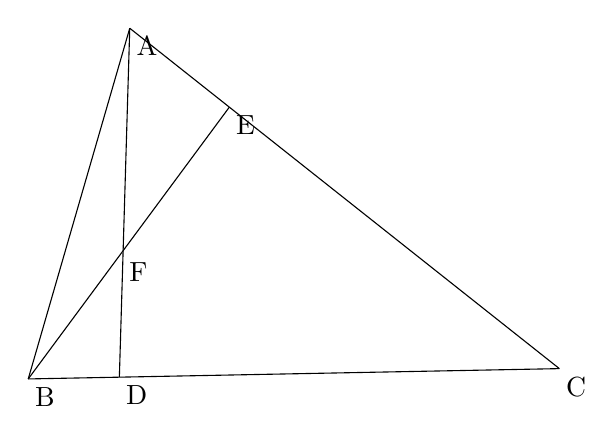
\begin{tikzpicture}[x=0.75pt,y=0.75pt,yscale=-1,xscale=1]
%uncomment if require: \path (0,300); %set diagram left start at 0, and has height of 300

%Straight Lines [id:da7675617641029677] 
\draw    (248.91,41.03) -- (200,210) ;
%Straight Lines [id:da08477900268519623] 
\draw    (248.91,41.03) -- (455.91,205.03) ;
%Straight Lines [id:da9475888247486965] 
\draw    (455.91,205.03) -- (200,210) ;
%Straight Lines [id:da019733232113179566] 
\draw    (248.91,41.03) -- (243.91,209.03) ;
%Straight Lines [id:da6042356170051348] 
\draw    (200,210) -- (296.91,79.03) ;

% Text Node
\draw (250.91,44.03) node [anchor=north west][inner sep=0.75pt]   [align=left] {A};
% Text Node
\draw (202,213) node [anchor=north west][inner sep=0.75pt]   [align=left] {B};
% Text Node
\draw (457.91,208.03) node [anchor=north west][inner sep=0.75pt]   [align=left] {C};
% Text Node
\draw (245.91,212.03) node [anchor=north west][inner sep=0.75pt]   [align=left] {D};
% Text Node
\draw (298.91,82.03) node [anchor=north west][inner sep=0.75pt]   [align=left] {E};
% Text Node
\draw (247.46,152.52) node [anchor=north west][inner sep=0.75pt]   [align=left] {F};


\end{tikzpicture}
   
\end{minipage}
\begin{minipage}{0.5\linewidth}
    First, let $C=1$:\\
    Since $C$ equals 1, $B$ must equal 5 and $A$ must equal 4.\\
    As a result, by adding $B$ and $C$, $D$ must be 6.\\
    Therefore $AF:FD=6:4=3:2$
\end{minipage}

\section{Angle Bisector}


\subsection{Definition}
A ray that bisects an angle.

\subsection{Angle Bisector  Theorem}


If AD bisects $\angle A$, then

$$\frac{BD}{CD}=\frac{AB}{AC}$$\\\\




\tikzset{every picture/.style={line width=0.75pt}} %set default line width to 0.75pt        

\begin{tikzpicture}[x=0.75pt,y=0.75pt,yscale=-1,xscale=1]
%uncomment if require: \path (0,300); %set diagram left start at 0, and has height of 300

%Shape: Triangle [id:dp23420178669904668] 
\draw   (204.02,76.15) -- (548.2,200.08) -- (176,200.08) -- cycle ;
%Straight Lines [id:da10521333010274803] 
\draw    (204.02,76.15) -- (291.16,249.4) ;
%Straight Lines [id:da8232632334372048] 
\draw    (291.16,249.4) -- (176,200.08) ;
%Straight Lines [id:da8021364977010002] 
\draw    (235.26,219.77) -- (230.06,231.63) ;
%Straight Lines [id:da7737510285253735] 
\draw    (239.73,221.28) -- (234.52,233.14) ;
%Straight Lines [id:da43087736985352687] 
\draw    (182.19,146.27) -- (194.17,150.75) ;
%Straight Lines [id:da33230006794261135] 
\draw    (183.37,141.63) -- (195.35,146.12) ;

% Text Node
\draw (188.71,49.12) node [anchor=north west][inner sep=0.75pt]    {$A$};
% Text Node
\draw (200.72,100.71) node [anchor=north west][inner sep=0.75pt]  [font=\footnotesize]  {$\frac{A}{2}$};
% Text Node
\draw (253.92,204.31) node [anchor=north west][inner sep=0.75pt]  [font=\footnotesize]  {$\frac{A}{2}$};
% Text Node
\draw (225.92,92.31) node [anchor=north west][inner sep=0.75pt]  [font=\footnotesize]  {$\frac{A}{2}$};
% Text Node
\draw (461.6,65.4) node [anchor=north west][inner sep=0.75pt]    {$ \begin{array}{l}
ADC=EDB\\
\\
\frac{BD}{DC} =\frac{BE}{AC} =\frac{AB}{AC}
\end{array}$};
% Text Node
\draw (155.21,200.62) node [anchor=north west][inner sep=0.75pt]    {$B$};
% Text Node
\draw (550.71,197.12) node [anchor=north west][inner sep=0.75pt]    {$C$};
% Text Node
\draw (267.21,177.62) node [anchor=north west][inner sep=0.75pt]    {$D$};
% Text Node
\draw (285.71,261.62) node [anchor=north west][inner sep=0.75pt]    {$E$};


\end{tikzpicture}



\vspace{60px}

\subsection{Theorem}
Angle bisectors of a trinagle are concurrent, the point is called the incenter of the triangle.\\
\\
Proof 1:\\
$$\frac{AF}{FB}\times\frac{BD}{DC}\times\frac{CE}{EA}$$
\begin{align*}
&=\frac{b}{a}\times\frac{c}{b}\times\frac{a}{c}\\
&=1
\end{align*}
By using Ceva's Inverse Theorem (ref. 3.5, 3.6), we can state that $AD$, $BE$, and $CF$ are concurrent!\\
\\
Proof 2:



\tikzset{every picture/.style={line width=0.75pt}} %set default line width to 0.75pt        

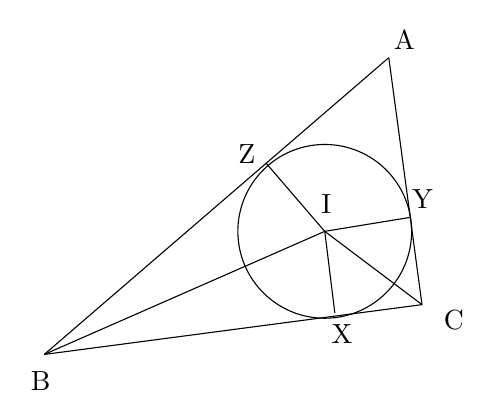
\begin{tikzpicture}[x=0.75pt,y=0.75pt,yscale=-1,xscale=1]
%uncomment if require: \path (0,300); %set diagram left start at 0, and has height of 300

%Shape: Circle [id:dp03363624454868308] 
\draw   (166,172.86) .. controls (166,149.74) and (184.74,131) .. (207.86,131) .. controls (230.98,131) and (249.72,149.74) .. (249.72,172.86) .. controls (249.72,195.98) and (230.98,214.72) .. (207.86,214.72) .. controls (184.74,214.72) and (166,195.98) .. (166,172.86) -- cycle ;
%Straight Lines [id:da16702483763259202] 
\draw    (72.72,232.17) -- (238.72,89.17) ;
%Straight Lines [id:da017342402565662107] 
\draw    (254.72,208.17) -- (238.72,89.17) ;
%Straight Lines [id:da34842330322080173] 
\draw    (254.72,208.17) -- (72.72,232.17) ;
%Straight Lines [id:da440457276206375] 
\draw    (72.72,232.17) -- (207.86,172.86) ;
%Straight Lines [id:da6374694696980359] 
\draw    (207.86,172.86) -- (254.72,208.17) ;
%Straight Lines [id:da6546015267230736] 
\draw    (212.72,212.17) -- (207.86,172.86) ;
%Straight Lines [id:da7915018804006162] 
\draw    (179.72,140.17) -- (207.86,172.86) ;
%Straight Lines [id:da4411219242332338] 
\draw    (248.72,166.17) -- (207.86,172.86) ;

% Text Node
\draw (240,75) node [anchor=north west][inner sep=0.75pt]   [align=left] {A};
% Text Node
\draw (65,239) node [anchor=north west][inner sep=0.75pt]   [align=left] {B};
% Text Node
\draw (264,210) node [anchor=north west][inner sep=0.75pt]   [align=left] {C};
% Text Node
\draw (209.86,216.72) node [anchor=north west][inner sep=0.75pt]   [align=left] {X};
% Text Node
\draw (248.72,151.67) node [anchor=north west][inner sep=0.75pt]   [align=left] {Y};
% Text Node
\draw (165,130) node [anchor=north west][inner sep=0.75pt]   [align=left] {Z};
% Text Node
\draw (205,154) node [anchor=north west][inner sep=0.75pt]   [align=left] {I};


\end{tikzpicture}\\
Let $I$ be the intersection of angle bisector from $B$ and $C$, we only need to show $AI$ also bisects $\angle A$.\\
Draw $IX$,$IY$,$IZ$ perpendicular to $BC,CA,AB$.\\
By hypotenuse-side congruence, $\triangle BIX \cong \triangle BIZ$, $\triangle CIX \cong \triangle CIY$.\\
Therefore, $IZ=IX=IY$.\\
Thus, $\triangle AIY \cong \triangle AIZ$, and $AI$ is the angle bisector from $A$.

\subsection{Theorem}
In $\triangle ABC$ with incenter I,  $\angle BIC = 90^{\circ}+\frac{1}{2}\angle A$


\begin{minipage}{0.4\linewidth}

\tikzset{every picture/.style={line width=0.75pt}} %set default line width to 0.75pt        

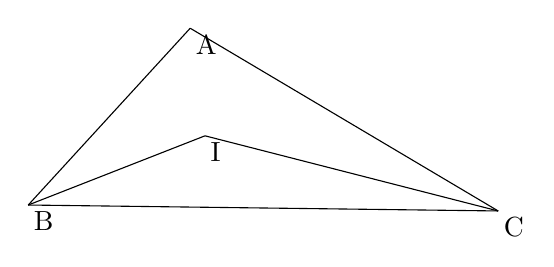
\begin{tikzpicture}[x=0.75pt,y=0.75pt,yscale=-.71,xscale=.71]
%uncomment if require: \path (0,300); %set diagram left start at 0, and has height of 300

%Straight Lines [id:da5905118684092199] 
\draw    (124,172) -- (442.91,176.03) ;
%Straight Lines [id:da9618382085114188] 
\draw    (124,172) -- (233.91,52.03) ;
%Straight Lines [id:da13878852480396842] 
\draw    (233.91,52.03) -- (442.91,176.03) ;
%Straight Lines [id:da09073327189026714] 
\draw    (243.96,125.03) -- (124,172) ;
%Straight Lines [id:da05856932878848253] 
\draw    (243.96,125.03) -- (442.91,176.03) ;

% Text Node
\draw (235.91,55.03) node [anchor=north west][inner sep=0.75pt]   [align=left] {A};
% Text Node
\draw (126,175) node [anchor=north west][inner sep=0.75pt]   [align=left] {B};
% Text Node
\draw (444.91,179.03) node [anchor=north west][inner sep=0.75pt]   [align=left] {C};
% Text Node
\draw (245.96,128.03) node [anchor=north west][inner sep=0.75pt]   [align=left] {I};


\end{tikzpicture}
\end{minipage}
\begin{minipage}{0.2\linewidth}
    \begin{align*}
        \angle I &= 180^\circ-\frac{1}{2}\angle B-\frac{1}{2}\angle C-\frac{1}{2}\angle A+\frac{1}{2}\angle A\\
        &=180^\circ-\frac{1}{2}(\angle A+\angle B+\angle C)+\frac{1}{2}\angle A\\
        &=90^\circ +\frac{1}{2}\angle A
    \end{align*}
\end{minipage}
\pagebreak

\subsection{Theorem}
In $\triangle ABC$ with incenter I, the circumcenter of $\triangle BIC$ is the mid point of the arc $\overset{\LARGE\frown}{BC}$.



\tikzset{every picture/.style={line width=0.75pt}} %set default line width to 0.75pt        

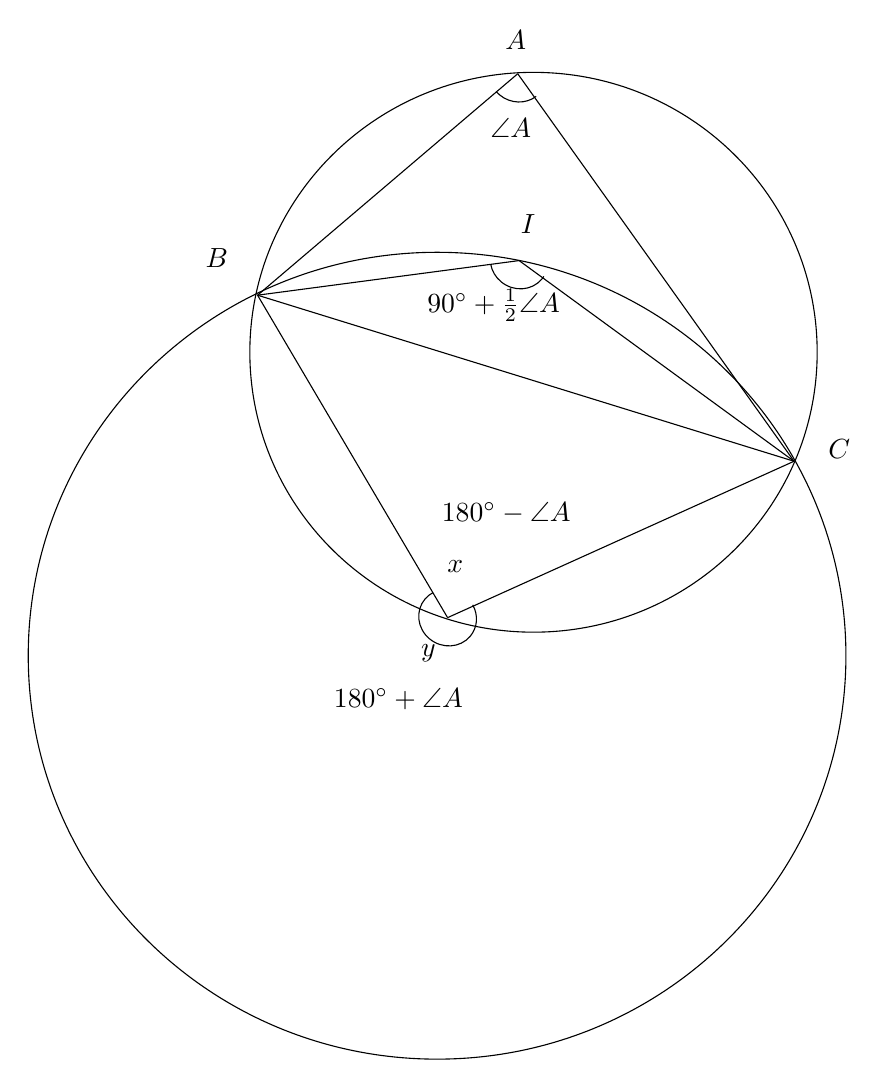
\begin{tikzpicture}[x=0.75pt,y=0.75pt,yscale=-1,xscale=1]
%uncomment if require: \path (0,515); %set diagram left start at 0, and has height of 515

%Shape: Ellipse [id:dp8341671878060917] 
\draw   (114.2,309.3) .. controls (114.2,201.95) and (202.39,114.93) .. (311.18,114.93) .. controls (419.97,114.93) and (508.16,201.95) .. (508.16,309.3) .. controls (508.16,416.64) and (419.97,503.67) .. (311.18,503.67) .. controls (202.39,503.67) and (114.2,416.64) .. (114.2,309.3) -- cycle ;
%Shape: Ellipse [id:dp19642093522126958] 
\draw   (220.97,163.1) .. controls (220.97,88.62) and (282.16,28.24) .. (357.64,28.24) .. controls (433.12,28.24) and (494.31,88.62) .. (494.31,163.1) .. controls (494.31,237.58) and (433.12,297.96) .. (357.64,297.96) .. controls (282.16,297.96) and (220.97,237.58) .. (220.97,163.1) -- cycle ;
%Straight Lines [id:da22666611648945834] 
\draw    (224.69,135.6) -- (483.16,215.61) ;
%Straight Lines [id:da5199610100088321] 
\draw    (224.69,135.6) -- (350.71,118.93) ;
%Straight Lines [id:da6381171376392452] 
\draw    (224.69,135.6) -- (350.04,28.91) ;
%Straight Lines [id:da5927231246625995] 
\draw    (350.04,28.91) -- (483.16,215.61) ;
%Straight Lines [id:da6732922234415006] 
\draw    (350.71,118.93) -- (483.16,215.61) ;
%Straight Lines [id:da42612706751497575] 
\draw    (224.69,135.6) -- (316.25,290.96) ;
%Straight Lines [id:da19197914127659788] 
\draw    (316.25,290.96) -- (483.16,215.61) ;
%Shape: Arc [id:dp7439648235097325] 
\draw  [draw opacity=0] (328.35,284.81) .. controls (331.08,289.64) and (330.78,295.67) .. (327.11,299.98) .. controls (322.3,305.61) and (313.54,306.14) .. (307.54,301.16) .. controls (301.55,296.18) and (300.59,287.57) .. (305.4,281.94) .. controls (306.49,280.65) and (307.8,279.63) .. (309.23,278.89) -- (316.25,290.96) -- cycle ; \draw   (328.35,284.81) .. controls (331.08,289.64) and (330.78,295.67) .. (327.11,299.98) .. controls (322.3,305.61) and (313.54,306.14) .. (307.54,301.16) .. controls (301.55,296.18) and (300.59,287.57) .. (305.4,281.94) .. controls (306.49,280.65) and (307.8,279.63) .. (309.23,278.89) ;  
%Shape: Arc [id:dp36590206271152703] 
\draw  [draw opacity=0] (362.61,126.54) .. controls (362.3,127.02) and (361.95,127.49) .. (361.57,127.94) .. controls (356.76,133.58) and (348,134.11) .. (342.01,129.13) .. controls (339.29,126.87) and (337.6,123.86) .. (337.02,120.72) -- (350.71,118.93) -- cycle ; \draw   (362.61,126.54) .. controls (362.3,127.02) and (361.95,127.49) .. (361.57,127.94) .. controls (356.76,133.58) and (348,134.11) .. (342.01,129.13) .. controls (339.29,126.87) and (337.6,123.86) .. (337.02,120.72) ;  
%Shape: Arc [id:dp6742092205856316] 
\draw  [draw opacity=0] (358.93,39.79) .. controls (353.95,43.61) and (346.58,43.47) .. (341.33,39.11) .. controls (340.72,38.6) and (340.15,38.05) .. (339.64,37.46) -- (350.04,28.91) -- cycle ; \draw   (358.93,39.79) .. controls (353.95,43.61) and (346.58,43.47) .. (341.33,39.11) .. controls (340.72,38.6) and (340.15,38.05) .. (339.64,37.46) ;  

% Text Node
\draw (198.41,111.99) node [anchor=north west][inner sep=0.75pt]    {$B$};
% Text Node
\draw (498.46,204.01) node [anchor=north west][inner sep=0.75pt]    {$C$};
% Text Node
\draw (314.87,262.24) node [anchor=north west][inner sep=0.75pt]    {$x$};
% Text Node
\draw (335.58,48.98) node [anchor=north west][inner sep=0.75pt]    {$\angle A$};
% Text Node
\draw (305.2,131.33) node [anchor=north west][inner sep=0.75pt]    {$90^\circ +\frac{1}{2} \angle A$};
% Text Node
\draw (342.78,6.98) node [anchor=north west][inner sep=0.75pt]    {$A$};
% Text Node
\draw (350.33,95.73) node [anchor=north west][inner sep=0.75pt]    {$I$};
% Text Node
\draw (312.24,233.98) node [anchor=north west][inner sep=0.75pt]    {$180^\circ -\angle A$};
% Text Node
\draw (260.24,323.65) node [anchor=north west][inner sep=0.75pt]    {$180^\circ +\angle A$};
% Text Node
\draw (302.2,302.57) node [anchor=north west][inner sep=0.75pt]    {$y$};


\end{tikzpicture}\\
Since $ABxC$ is a cyclic quadrilateral, we know that $\angle A+\angle x=180^\circ$ (opposite angles add up to $180^\circ$). Therefore $x=180^\circ -\angle A$, and $\angle y=360^\circ - (180^\circ -\angle A)=180^\circ +\angle A$.\\
By Theorem 5.4, $\angle BIC=90^\circ +\frac{1}{2}\angle A$. Since the circumcenter of $\triangle BIC$ is on the perpendicular bisector of $BC$, and $\angle y = 2\angle I$, the circumcenter of BIC must be on the midpoint of arc BC.


\pagebreak

\section{Median}

\subsection{Definition}
A line segment joins a vertex to the midpoint of the opposite side.

\subsection{Theorem}
Medians of triangle are concurrent. The point is called the centroid of the triangle.\\
Proof: This is a simple corollary of Inverse Ceva's Theorem.

\subsection{Theorem}
In $\triangle ABC$ with centroid G and A' as the midpoint of BC, AG=2GA'.




\tikzset{every picture/.style={line width=0.75pt}} %set default line width to 0.75pt        

\begin{tikzpicture}[x=0.75pt,y=0.75pt,yscale=-1,xscale=1]
%uncomment if require: \path (0,300); %set diagram left start at 0, and has height of 300

%Shape: Triangle [id:dp1962076307937537] 
\draw   (182.6,69) -- (264.6,167) -- (40,167) -- cycle ;
%Straight Lines [id:da3638340674911742] 
\draw    (182.6,69) -- (145.8,167.4) ;

% Text Node
\draw (140,173.2) node [anchor=north west][inner sep=0.75pt]    {$A'$};
% Text Node
\draw (177.2,50.4) node [anchor=north west][inner sep=0.75pt]    {$A$};
% Text Node
\draw (22.8,169.6) node [anchor=north west][inner sep=0.75pt]    {$B$};
% Text Node
\draw (268.4,166.8) node [anchor=north west][inner sep=0.75pt]    {$C$};
% Text Node
\draw (271.2,185.6) node [anchor=north west][inner sep=0.75pt]   [align=left] {{\footnotesize m}};
% Text Node
\draw (22.8,186.8) node [anchor=north west][inner sep=0.75pt]   [align=left] {{\footnotesize m}};
% Text Node
\draw (192,64.4) node [anchor=north west][inner sep=0.75pt]   [align=left] {{\footnotesize m}};
% Text Node
\draw (136.8,196) node [anchor=north west][inner sep=0.75pt]   [align=left] {{\footnotesize 2m}};
% Text Node
\draw (258,73) node [anchor=north west][inner sep=0.75pt]    {$A:A'=1:2$};


\end{tikzpicture}\\
Proof: This is a simple corollary of the barycentric coordinate.


\subsection{Median Length Formula}

In $\triangle ABC$ with median AA'=m, then $\frac{1}{2}m^2=b^2+c^2-\frac{1}{2}a^2$


\tikzset{every picture/.style={line width=0.75pt}} %set default line width to 0.75pt        

\begin{tikzpicture}[x=0.75pt,y=0.75pt,yscale=-1,xscale=1]
%uncomment if require: \path (0,389); %set diagram left start at 0, and has height of 389

%Straight Lines [id:da28332928208796315] 
\draw    (128.06,259.03) -- (364.06,261.03) ;
%Straight Lines [id:da647118791580753] 
\draw    (285.96,124.03) -- (128.06,259.03) ;
%Straight Lines [id:da4424909815278173] 
\draw    (285.96,124.03) -- (364.06,261.03) ;
%Straight Lines [id:da11044244004039627] 
\draw    (285.96,124.03) -- (246.06,260.03) ;

% Text Node
\draw (287.96,127.03) node [anchor=north west][inner sep=0.75pt]   [align=left] {A};
% Text Node
\draw (130.06,262.03) node [anchor=north west][inner sep=0.75pt]   [align=left] {B};
% Text Node
\draw (366.06,264.03) node [anchor=north west][inner sep=0.75pt]   [align=left] {C};
% Text Node
\draw (248.06,263.03) node [anchor=north west][inner sep=0.75pt]   [align=left] {A'};


\end{tikzpicture}\\
Proof: This is a simple corollary of Stewart's Theorem.
\pagebreak

\section{Height}

\subsection{Definition}
The height of a triangle is the perpendicular line from one vertex to its opposite side, which is arbitrarily denoted as the base. For example, in the following diagram, the height is the highlighted portion of the triangle below.
\vspace{20px}

\subsection{Theorem}

Heights of triangle are concurrent. The point is called the orthocenter of the triangle.




\tikzset{every picture/.style={line width=0.75pt}} %set default line width to 0.75pt        

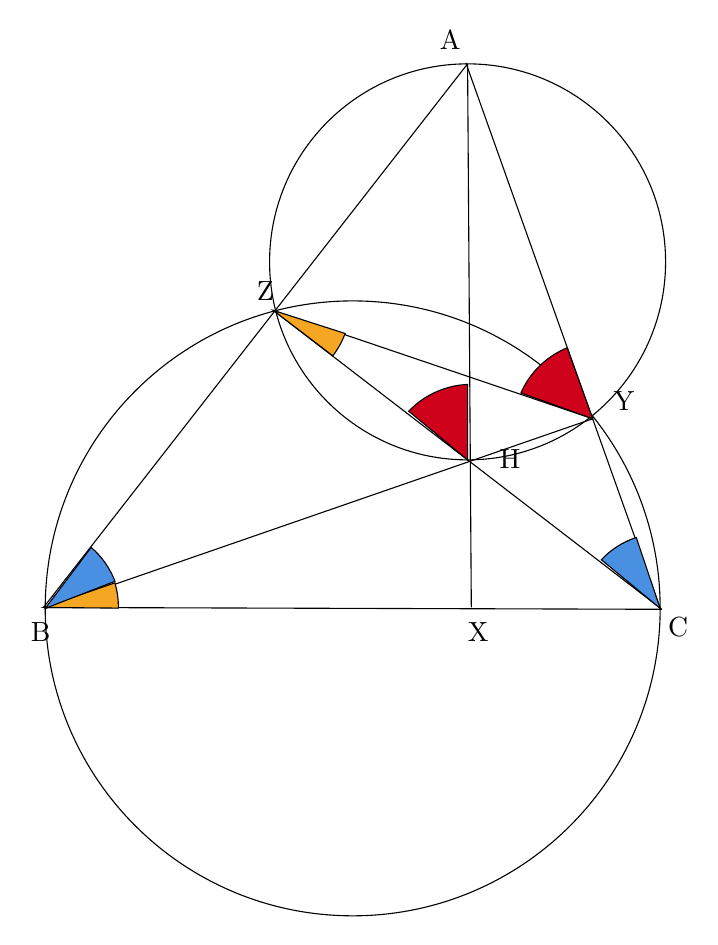
\begin{tikzpicture}[x=0.75pt,y=0.75pt,yscale=-.9,xscale=.9]
%uncomment if require: \path (0,585); %set diagram left start at 0, and has height of 585

%Straight Lines [id:da8043865334309586] 
\draw    (321.2,72.07) -- (94.2,363.07) ;
%Straight Lines [id:da9561527315905409] 
\draw    (425.2,364.07) -- (94.2,363.07) ;
%Straight Lines [id:da27192801087570384] 
\draw    (320.29,71.57) -- (424.29,363.57) ;
%Straight Lines [id:da0289227455950003] 
\draw    (388.2,262.07) -- (95.1,363.57) ;
%Straight Lines [id:da7841077574593995] 
\draw    (217.2,204.07) -- (425.2,364.07) ;
%Shape: Circle [id:dp3927232729466583] 
\draw   (95.1,363.57) .. controls (95.1,272.66) and (168.79,198.97) .. (259.7,198.97) .. controls (350.6,198.97) and (424.29,272.66) .. (424.29,363.57) .. controls (424.29,454.47) and (350.6,528.16) .. (259.7,528.16) .. controls (168.79,528.16) and (95.1,454.47) .. (95.1,363.57) -- cycle ;
%Straight Lines [id:da9225848977880937] 
\draw    (321.2,72.07) -- (323.2,362.97) ;
%Shape: Circle [id:dp4032337912717612] 
\draw   (215.2,178.07) .. controls (215.2,119.52) and (262.65,72.07) .. (321.2,72.07) .. controls (379.74,72.07) and (427.2,119.52) .. (427.2,178.07) .. controls (427.2,236.61) and (379.74,284.07) .. (321.2,284.07) .. controls (262.65,284.07) and (215.2,236.61) .. (215.2,178.07) -- cycle ;
%Straight Lines [id:da4705045743399143] 
\draw    (217.2,204.07) -- (388.2,262.07) ;
%Shape: Pie [id:dp38574678633740933] 
\draw  [fill={rgb, 255:red, 245; green, 166; blue, 35 }  ,fill opacity=1 ] (132.38,349.91) .. controls (133.65,354.17) and (134.31,358.71) .. (134.27,363.43) -- (94.2,363.07) -- cycle ;
%Shape: Pie [id:dp6153306022713583] 
\draw  [fill={rgb, 255:red, 245; green, 166; blue, 35 }  ,fill opacity=1 ] (255.65,216.41) .. controls (254.11,220.57) and (251.92,224.61) .. (249.06,228.36) -- (217.2,204.07) -- cycle ;
%Shape: Pie [id:dp9417310149274456] 
\draw  [fill={rgb, 255:red, 74; green, 144; blue, 226 }  ,fill opacity=1 ] (119.7,330.95) .. controls (125.16,335.63) and (129.63,341.77) .. (132.46,349.07) -- (95.1,363.57) -- cycle ;
%Shape: Pie [id:dp08427696631981951] 
\draw  [fill={rgb, 255:red, 74; green, 144; blue, 226 }  ,fill opacity=1 ] (392.81,337.53) .. controls (397.72,332.29) and (404.06,328.1) .. (411.48,325.6) -- (424.29,363.57) -- cycle ;
%Shape: Pie [id:dp24531417078429518] 
\draw  [fill={rgb, 255:red, 208; green, 2; blue, 27 }  ,fill opacity=1 ] (289.71,258.03) .. controls (294.63,252.79) and (300.97,248.6) .. (308.39,246.1) .. controls (312.65,244.66) and (316.96,243.88) .. (321.2,243.7) -- (321.2,284.07) -- cycle ;
%Shape: Pie [id:dp5760571202545177] 
\draw  [fill={rgb, 255:red, 208; green, 2; blue, 27 }  ,fill opacity=1 ] (349.75,248.24) .. controls (352.6,241.64) and (357.14,235.55) .. (363.28,230.68) .. controls (366.8,227.89) and (370.59,225.7) .. (374.52,224.09) -- (388.2,262.07) -- cycle ;

% Text Node
\draw (305,53) node [anchor=north west][inner sep=0.75pt]   [align=left] {A};
% Text Node
\draw (86,370) node [anchor=north west][inner sep=0.75pt]   [align=left] {B};
% Text Node
\draw (320,370) node [anchor=north west][inner sep=0.75pt]   [align=left] {X};
% Text Node
\draw (427.2,367.07) node [anchor=north west][inner sep=0.75pt]   [align=left] {C};
% Text Node
\draw (337,277) node [anchor=north west][inner sep=0.75pt]   [align=left] {H};
% Text Node
\draw (398,246) node [anchor=north west][inner sep=0.75pt]   [align=left] {Y};
% Text Node
\draw (207,187) node [anchor=north west][inner sep=0.75pt]   [align=left] {Z};


\end{tikzpicture}\\
To prove that the heights of triangles are concurrent, we will have to draw a line that passes through point $H$ and prove that it intersects $BC$ at a $90^\circ$ angle.\\
Since $\angle BZC$ and $\angle BYC$ are right angles, we know that $BC$ is the diameter of the large circle. \\
Since $\angle HZA$ and $\angle HYA$ are right angles,   we know that $AH$ is the diameter of the smaller circle. \\
We know that $\angle ZBX=\angle YBC+\angle ZBY=\angle YZC+\angle YCZ=\angle AY=\angle AHZ$. Therefore, $\angle ZBX+\angle ZHX=180^\circ$, making it a cyclic quadrilateral. \\
Since $XBZH$ is a cyclic quadrilateral, with $\angle BZC=90^\circ$, $\angle BXH$ must be $90^\circ$, therefore making $AX$ the height of $\triangle ABC$, and thus concurrent with the two other heights.




\pagebreak

\subsection{Theorem}

In $\triangle ABC$ with orthocenter H, A' the midpoint of BC, and the circumcenter O, AH=2OA'.





\tikzset{every picture/.style={line width=0.75pt}} %set default line width to 0.75pt        

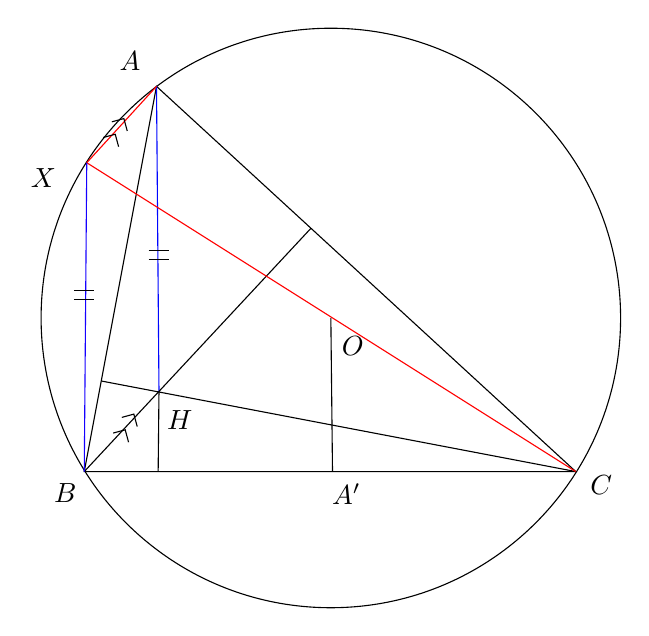
\begin{tikzpicture}[x=0.75pt,y=0.75pt,yscale=-1,xscale=1]
%uncomment if require: \path (0,300); %set diagram left start at 0, and has height of 300

%Shape: Circle [id:dp8341671878060917] 
\draw   (50.6,149.8) .. controls (50.6,72.7) and (113.1,10.2) .. (190.2,10.2) .. controls (267.3,10.2) and (329.8,72.7) .. (329.8,149.8) .. controls (329.8,226.9) and (267.3,289.4) .. (190.2,289.4) .. controls (113.1,289.4) and (50.6,226.9) .. (50.6,149.8) -- cycle ;
%Shape: Triangle [id:dp8889012913980656] 
\draw   (106.2,38.2) -- (308.2,223.8) -- (71.4,223.8) -- cycle ;
%Straight Lines [id:da671414338683672] 
\draw    (190.2,149.8) -- (191,223.8) ;
%Straight Lines [id:da6452369633817994] 
\draw [color={rgb, 255:red, 0; green, 6; blue, 255 }  ,draw opacity=1 ]   (106.2,38.2) -- (107.4,185) ;
%Straight Lines [id:da22750638406962942] 
\draw    (71.4,223.8) -- (180.6,106.6) ;
%Straight Lines [id:da7641975173619191] 
\draw    (79.8,180.2) -- (308.2,223.8) ;
%Straight Lines [id:da695640988124588] 
\draw [color={rgb, 255:red, 255; green, 0; blue, 0 }  ,draw opacity=1 ]   (72.6,75) -- (308.2,223.8) ;
%Straight Lines [id:da14325005216249664] 
\draw [color={rgb, 255:red, 21; green, 0; blue, 255 }  ,draw opacity=1 ]   (72.6,75) -- (71.4,223.8) ;
%Straight Lines [id:da22702197265707058] 
\draw [color={rgb, 255:red, 255; green, 0; blue, 0 }  ,draw opacity=1 ][fill={rgb, 255:red, 255; green, 0; blue, 0 }  ,fill opacity=1 ]   (72.6,75) -- (106.2,38.2) ;
%Shape: Right Angle [id:dp6837172941907061] 
\draw   (84.69,55.3) -- (90.48,53.72) -- (92.11,59.7) ;
%Shape: Right Angle [id:dp050991571581555206] 
\draw   (80.53,62.85) -- (86.32,61.28) -- (87.94,67.26) ;
%Shape: Right Angle [id:dp6232542700274768] 
\draw   (89.49,197.7) -- (95.28,196.12) -- (96.91,202.1) ;
%Shape: Right Angle [id:dp4892912803487397] 
\draw   (85.33,205.25) -- (91.12,203.68) -- (92.74,209.66) ;
%Straight Lines [id:da11661336366120634] 
\draw    (66.4,136.6) -- (76.2,136.6) ;
%Straight Lines [id:da11214858542911155] 
\draw    (66.4,141) -- (76.2,141) ;
%Straight Lines [id:da8059674020255574] 
\draw    (102.4,117.4) -- (112.2,117.4) ;
%Straight Lines [id:da6768483822078768] 
\draw    (102.4,121.8) -- (112.2,121.8) ;
%Straight Lines [id:da49026108799564727] 
\draw    (107.4,185) -- (107,223.8) ;

% Text Node
\draw (87.2,20.2) node [anchor=north west][inner sep=0.75pt]    {$A$};
% Text Node
\draw (55.6,228.2) node [anchor=north west][inner sep=0.75pt]    {$B$};
% Text Node
\draw (314,224.6) node [anchor=north west][inner sep=0.75pt]    {$C$};
% Text Node
\draw (194.2,157.6) node [anchor=north west][inner sep=0.75pt]    {$O$};
% Text Node
\draw (110,193) node [anchor=north west][inner sep=0.75pt]    {$H$};
% Text Node
\draw (189.6,228.6) node [anchor=north west][inner sep=0.75pt]    {$A'$};
% Text Node
\draw (44.4,76.8) node [anchor=north west][inner sep=0.75pt]    {$X$};


\end{tikzpicture}\\
Since $XAC$ is a triangle with $XC$, the diameter of the circle, as it's base, $\angle XAC$ is $90^\circ$.\\
We also know that the extended line, $BH$, goes through the orthocenter, and therefore must form a $90^\circ$ angle when intersecting $AC$.\\
Therefore, $XA//BH$.\\\\
Since $CX$ is the diameter of the circle, $\angle XBC$ must be $90^\circ$.\\
Since $AH$ passes through the orthocenter, it intersects $BC$ at a $90^\circ$ angle.\\
Therefore, $XB//AH$.\\\\
Therefore, $AXBH$ is a parallelogram.\\\\
"A' the midpoint of BC" = Homothety!\\
$A'O=\frac{1}{2} BX$\\
$BX=AH$\\
$\therefore \ A'O=\frac{1}{2} AH$


\pagebreak
\subsection{Theorem:}
O the circumcenter,G the centroid,H the orthocenter are collinear. This line is called the Euler line of the triangle.



\tikzset{every picture/.style={line width=0.75pt}} %set default line width to 0.75pt        

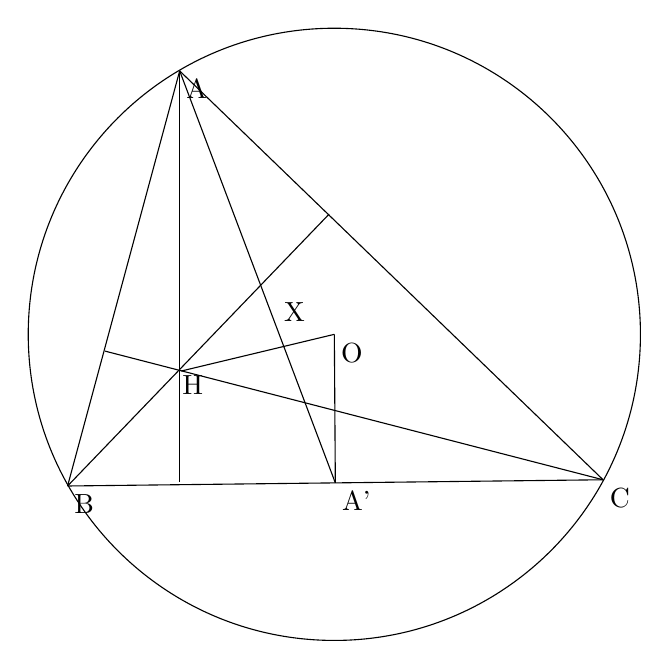
\begin{tikzpicture}[x=0.75pt,y=0.75pt,yscale=-1,xscale=1]
%uncomment if require: \path (0,389); %set diagram left start at 0, and has height of 389

%Shape: Circle [id:dp9162436210882785] 
\draw   (138,201.48) .. controls (138,120.03) and (204.03,54) .. (285.48,54) .. controls (366.93,54) and (432.96,120.03) .. (432.96,201.48) .. controls (432.96,282.93) and (366.93,348.96) .. (285.48,348.96) .. controls (204.03,348.96) and (138,282.93) .. (138,201.48) -- cycle ;
%Straight Lines [id:da7741878669053166] 
\draw    (156.96,274.55) -- (210.96,74.55) ;
%Straight Lines [id:da3851763576282945] 
\draw    (414.96,271.55) -- (156.96,274.55) ;
%Straight Lines [id:da10655267360857046] 
\draw    (210.96,74.55) -- (414.96,271.55) ;
%Straight Lines [id:da08513658544714886] 
\draw    (285.96,273.05) -- (285.48,201.48) ;
%Straight Lines [id:da351408405309773] 
\draw    (210.96,272.55) -- (210.96,74.55) ;
%Straight Lines [id:da09103761919117792] 
\draw    (282.96,143.55) -- (156.96,274.55) ;
%Straight Lines [id:da9902153949193253] 
\draw    (174.96,209.55) -- (414.96,271.55) ;
%Straight Lines [id:da22691628499294447] 
\draw    (210.96,74.55) -- (285.96,273.05) ;
%Straight Lines [id:da0130777312781869] 
\draw    (285.48,201.48) -- (211.72,219.16) ;

% Text Node
\draw (212.96,77.55) node [anchor=north west][inner sep=0.75pt]   [align=left] {A};
% Text Node
\draw (158.96,277.55) node [anchor=north west][inner sep=0.75pt]   [align=left] {B};
% Text Node
\draw (416.96,274.55) node [anchor=north west][inner sep=0.75pt]   [align=left] {C};
% Text Node
\draw (211,220) node [anchor=north west][inner sep=0.75pt]   [align=left] {H};
% Text Node
\draw (287.48,204.48) node [anchor=north west][inner sep=0.75pt]   [align=left] {O};
% Text Node
\draw (287.96,276.05) node [anchor=north west][inner sep=0.75pt]   [align=left] {A'};
% Text Node
\draw (260,185) node [anchor=north west][inner sep=0.75pt]   [align=left] {X};

\end{tikzpicture}\\
Join $AA'$ and $OH$ and let the intersection be $X$.\\
 By Theorem 7.3, and by similar triangles, we know $A'X=2AX$.\\
 Then by Theorem 6.3, this $X$ must be $G$, therefore $O, G, H$ colinear.
\end{document}
